\section{Git remotes}
\begin{frame}[fragile]
  \slidetitle
  This section covers the following topics:
  \begin{itemize}
    \item Git remote repository concept
    \item Add remote repositories
    \item Synchronize with remote repositories
  \end{itemize}
\end{frame}

\subsection{Remote repositories}
\begin{frame}[fragile]
  \subslidetitle
  The \cmd{git remote} allows to manage remote repositories:
  \begin{lstlisting}
$ (*\textcolor[HTML]{0000AA}{git remote show}*)
origin

$ (*\textcolor[HTML]{0000AA}{git remote show origin}*)
* remote origin
  Fetch URL: https://github.com/neolynx/gitmoon.git
  Push  URL: https://github.com/neolynx/gitmoon.git
  HEAD branch: master
  Remote branch:
    master tracked
  Local branch configured for 'git pull':
    master merges with remote master
  Local ref configured for 'git push':
    master pushes to master (up to date)
\end{lstlisting}
  \vspace{1em}
  Note: the default remote is called \textbf{origin}
\end{frame}

\subsection{Git protocols}
\begin{frame}[fragile]
  \subslidetitle
  Git repositories can be accessed locally or over the network.
  \\
  \vspace{1em}
  Various protocols are supported:
  \begin{itemize}
  \opt{local}  {file system based}
  \opt{http[s]}{good for read only access without password}
  \opt{ssh}    {normally used for read-write access}
  \opt{git}    {git native protocol on port 9418}
  \opt{legacy} {ftp, rsync, ...}
  \end{itemize}
  \vspace{1em}
  %With ssh configured we are not prompt for our password on every request
  SSH provides us the possibility to authenticate without having to enter the password on every request.
\end{frame}

\subsection{Configure SSH access}
\begin{frame}[fragile]
  \subslidetitle
  Create a SSH key pair:
  \begin{lstlisting}
$ (*\textcolor[HTML]{0000AA}{ssh-keygen -f \textasciitilde/.ssh/id\_rsa\_workshop}*)
Generating public/private rsa key pair.
Enter passphrase (empty for no passphrase): (*\textcolor[HTML]{0000AA}{<enter>}*)
Enter same passphrase again: (*\textcolor[HTML]{0000AA}{<enter>}*)
Your identification has been saved in .../.ssh/id_rsa_workshop.
Your public key has been saved in .../.ssh/id_rsa_workshop.pub.
The key fingerprint is:
7e:f8:15:2a:b3:a2:9c:30:4e:c7:60:50:a4:d5:a9:82 user@host
The key's randomart image is:
+--[ RSA 2048]----+
|   . . .         |
|  . = = S        |
|   = X * X O o   |
...
\end{lstlisting}
\end{frame}

\subsection{Configure SSH access}
\begin{frame}[fragile]
  \subslidetitle
  Display your public key:
  \begin{lstlisting}
$ (*\textcolor[HTML]{0000AA}{cat \textasciitilde/.ssh/id\_rsa\_workshop.pub}*)
ssh-rsa AAAAB3NzaC1yc2EAAAADAQABAAABAQDOmt7Y4H51gc2m
GmZsFzES6shVLFLEJ/lFCTwyosWHYDaluK71nGCelp61oTocgf4N
HBwTZmo0EZ1k0RHYt8Q3LF8e5fbC+dXt5E35XtkVFuUC7IG2/6fm
NW41j3lw9UUVrOBDgx+QvvoCuRQaxNd4mRaLsRbj9WXt17hGuNNW
ioKPWLSpw/4KHJ34hCrnliAQJ+jlW/0ieOooFp057diCka6Jn7BW
jXHi8sWMxIfyPyV2+4Kt8OpChFNYjzaL5LMRRhMnvJ8zP5SFJB2q
HP50zPYQ+gKoSda7GZedZRgD7gT7ir/u8X9HSpNyTNTafhp9+3Aj
uUiYLTgtczTgYk/T user@host
\end{lstlisting}

  This whole output can be added to the SSH access keys
  section in the web frontend of your git appliance.
\end{frame}

\subsection{Exercises}
\begin{frame}[fragile]
  \subslidetitle
  \begin{exercise}
    \item Create a SSH key pair
    \item Configure SSH access in your git appliance
    \item Create a new private repository called \textbf{mygitmoon} in your git appliance
    \item Clone the new repository in your home \\
      (Hint: switch to your home directory first, by typing \cmd{cd})
    \item Go back to the original gitmoon project (\cmd{cd \textasciitilde/gitmoon})
  \end{exercise}
\end{frame}

\subsection{Adding a remote repository}
\begin{frame}[fragile]
  \subslidetitle
  Let's add the private repository as remote called \textbf{upstream}:
  \begin{lstlisting}
$ (*\textcolor[HTML]{0000AA}{git remote add upstream} \textcolor[HTML]{444444}{URL}*)
$ (*\textcolor[HTML]{0000AA}{git remote show}*)
origin
upstream
\end{lstlisting}
\vspace{1em}
\cmd{URL} stands for the url of your recent created repository in your git appliance
\vspace{1em}
\center 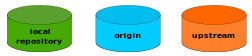
\includegraphics{diagrams/remote-add.pdf}
\end{frame}

\subsection{Pushing commits to a remote}
\begin{frame}[fragile]
  \subslidetitle
  Now, we can push our local commits to the \textbf{upstream} remote:
  \begin{lstlisting}
$ (*\textcolor[HTML]{0000AA}{git push upstream master}*)
git push upstream master
Counting objects: 6, done.
Delta compression using up to 2 threads.
Compressing objects: 100% (6/6), done.
Writing objects: 100% (6/6), 331.07 KiB | 0 bytes/s, done.
Total 6 (delta 0), reused 0 (delta 0)
remote: ...
To (*\textcolor[HTML]{444444}{URL}*)
 * [new branch]      master -> master
\end{lstlisting}
\vspace{-1.1em}
\center 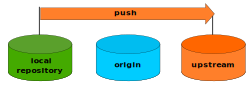
\includegraphics{diagrams/remote-push.pdf}
\end{frame}

\subsection{Pull request}
\begin{frame}[fragile]
  \subslidetitle
  Now, we can push our local branch \textbf{fix-title} to the \textbf{upstream} remote:
  \begin{lstlisting}
(*\textcolor[HTML]{18B2B2}{(master)}*) $ (*\textcolor[HTML]{0000AA}{git push upstream fix-title}*)
...
Total 3 (delta 2), reused 0 (delta 0)
remote:
remote: Create pull request for fix-title:
remote:   https://URL/mygitmoon/compare/commits?sourceBranch=refs/heads/fix-title
remote:
To (*\textcolor[HTML]{444444}{URL/mygitmoon.git}*)
 * [new branch]      fix-title -> fix-title
\end{lstlisting}
  Note: ensure the pull request reviewer has the appropriate permissions
  \newline
  Copy and paste the remote https:// URL in a browser to go on with the pull request
\end{frame}

\subsection{Pulling commits from a remote}
\begin{frame}[fragile]
  \subslidetitle
  In our \textbf{mygitmoon} project, these commits can now be pulled:
  \begin{lstlisting}
$ (*\textcolor[HTML]{0000AA}{cd \textasciitilde/mygitmoon}*)
$ (*\textcolor[HTML]{0000AA}{git pull}*)
remote: Counting objects: 6, done.
remote: Compressing objects: 100% (6/6), done.
remote: Total 6 (delta 0), reused 0 (delta 0)
Unpacking objects: 100% (6/6), done.
From (*\textcolor[HTML]{444444}{URL/mygitmoon.git}*)
 * [new branch]      master     -> origin/master
\end{lstlisting}
\center 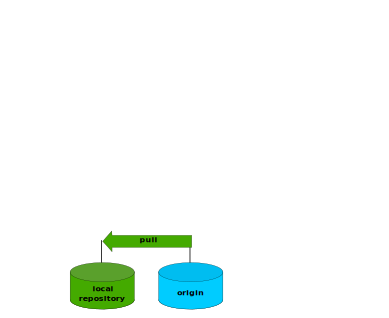
\includegraphics{diagrams/remote-pull.pdf}
\end{frame}

\subsection{Remote commands}
\begin{frame}[fragile]
  \subslidetitle
  The following commands operate on remote repositories:
  \begin{itemize}
    \item \cmd{git fetch} \\
      Downloads all branches from another repository
    \item \cmd{git pull --rebase} \\
      Does a \cmd{fetch} and then a {rebase} of the current branch onto a remote branch
    \item \cmd{git remote update} \\
      Does a \cmd{fetch} for all remotes
  \end{itemize}
\end{frame}

\subsection{Checkout a tracking branch}
\begin{frame}[fragile]
  \subslidetitle
  Once your remote is up to date, you have to checkout a specific local branch pointing to a remote branch:

  \begin{lstlisting}
(*\textcolor[HTML]{18B2B2}{(master)}*) $ (*\textcolor[HTML]{0000AA}{git checkout -b fix-title origin/fix-title --track}*)
Branch fix-title set up to track remote branch fix-title from origin.
Switched to a new branch 'fix-title'
\end{lstlisting}
  \vspace{1em}
  Note: you need to create a local branch pointing to one remote in order to push to this remote branch.

  \vspace{1em}
  Git does automatically setup the master branch to track the remote master branch.
\end{frame}

\subsection{Git appliances}
\begin{frame}[fragile]
  \subslidetitle
  There are various git appliances, providing the following features:
  \begin{itemize}
    \item Forking a repository
    \item Creating pull requests
    \item Offers branching models
  \end{itemize}
\end{frame}

\subsection{Branching models}
\begin{frame}[fragile]
  \subslidetitle
  A feature branch model looks like this:
  \center 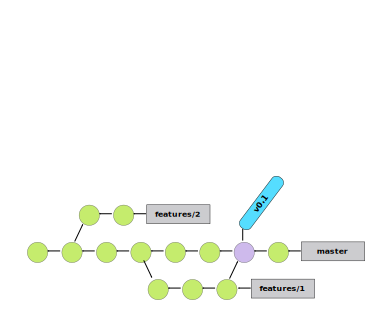
\includegraphics{diagrams/git-workflow.pdf}

  \vspace{2em}
  The idea is to not work directly on the master branch. Every change is made in a branch and gets merged into master eventually.
\end{frame}
